\section{Многоуровневая модель OSI (Open Systems Interconnection)}
Процесс передачи данных по компьютерной сети очень сложен, поэтому специалисты International Standards Organization решили разделить его на семь логических независимых уровней. Специалист на одном уровне может работать независимо от специалиста на другом уровне, не мешая друг другу.
\begin{table}[!h]
\begin{tabular}{|c|c|c|}
\hline
№ & Название уровня (layer) & Основная функция \\
\hline
\multirow{2}{*}{7} & \multirow{2}{*}{прикладной (application)} & взаимодействие программы пользователя \\
& & с сетевой подсистемой ОС (API) \\
\hline
\multirow{2}{*}{6} & уровень представления & \multirow{2}{*}{шифрование, сжатие, выбор кодировки}\\
 & (presentation) & \\
\hline
5 & сеансовый (session)  & установление соединения\\
\hline
4 & транспортный (transport)  & надежность доставки, реакция на потери\\
\hline
\multirow{3}{*}{3} & \multirow{3}{*}{сетевой (network)} & маршрутизация, объединение  \\
& & разнородных локальных сетей, \\
& & адресация в глобальной сети (IP) \\
\hline
\multirow{3}{*}{2} & \multirow{3}{*}{канальный (data link)} & связь между узлами одной локальной \\
& & сети, адресация в локальной сети \\
& & (МАС-адрес)\\
\hline
\multirow{2}{*}{1} & \multirow{2}{*}{физический (physical)} & физические характеристики каналов  \\
& & связи и передаваемых сигналов \\
\hline
\end{tabular}
\end{table}
\subsection{Прикладной уровень}
\emph{Субъекты взаимодействия:} пользовательская программа на передающем/принимающем компьютере; ОС.
\\\emph{Объекты взаимодействия:} Пользовательские данные, представленные в "родном" понятном виде для приемной и передающей программы.
\\\emph{Основные функции:} Вызов специальных функций ОС для работы с сетью (API). Программист не обязан знать о внутреннем устройстве
сети, для него передача данных по сети не отличается от сохранения в файл (просто надо вызвать нужную функцию API ОС).
\\\textbf{API} (интерфейс программирования приложений, интерфейс прикладного программирования) (англ. \emph{application programming interface}) — набор готовых классов, процедур, функций, структур и констант, предоставляемых приложением (библиотекой, сервисом) для использования во внешних программных продуктах. Используется программистами при написании всевозможных приложений.
\subsection{Уровень представления}
\emph{Субъекты взаимодействия:} специальное ПО для шифрования, сжатия, кодирования; ОС.
\\\emph{Объекты взаимодействия:} Закодированные пользовательские данные (пользовательская программа уже не может работать с такими данными без декодирования).
\\\emph{Основные функции:} Шифрование, сжатие, выбор кодировки, выбор способа представления порядка байт (little-endian, big-endian).
Каждый этап может выполняться несколько раз разными субъектами.
\subsection{Сеансовый уровень}
\emph{Субъекты взаимодействия:} ОС на компьютере-передатчике; ОС на компьютере-приемнике.
\\\emph{Объекты взаимодействия:} Служебные данные о об установке соединения: логины, пароли, сертификаты, цифровые подписи, пустые пакеты для проверки отсутствия обрывов связи, служебные пакеты с командами типа "запрос соединения", "подтверждение соединения", "разрыв соединения" (т.е. никакие пользовательские данные на этом уровне не передаются).
\\\emph{Основные функции:}
\begin{itemize}
\item Установление соединения (с возможной аутентификацией абонентов).
\item Отслеживание состояния соединения (возможное автопереподключение при обнаружении ошибок).
\item Реагирование на долгую неактивность сеанса связи (например, автоотсоединение по таймауту).
\item Принудительный разрыв соединения при окончании передачи (попутно освобождаются ресурсы ОС, которые хранят информацию о состоянии сеанса).
\end{itemize}
\subsection{Транспортный уровень}
\emph{Субъекты взаимодействия:} ОС; драйвер сетевой карты.
\\\emph{Объекты взаимодействия:} Пользовательские данные, снабженные служебными заголовками для обнаружения проблем передачи (контрольная сумма, порядковые номера фрагментов), служебные пакеты-подтверждения.
\\\emph{Основные функции:}
\begin{itemize}
  \item Отслеживание проблемных пакетов: искаженных, потерянных, пришедших в неверном порядке или дубликатов.
  \item Реакция на обнаружение проблемных пакетов (запрос повторной передачи или игнорирование, сбор целых пакетов из пришедших в разном порядке фрагментов).
  \item Реализация механизма повторной передачи (передается весь файл целиком или только проблемные части).
\end{itemize}
\subsection{Сетевой уровень}
\emph{Субъекты взаимодействия:} ОС; драйвер сетевой карты.
\\\emph{Объекты взаимодействия:} Данные, нарезанные на фрагменты, которые можно передавать в конкретной локальной сети (например, в
проводных сетях Fast Ethernet предельный размер фрагмента $\approx$ 1500 байт, а в сетях Wi-Fi он равен $\approx$ 8000 байт). Каждый фрагмент снабжается глобальным адресом (например, IP-адресом), который понятен в любой локальной сети, но при этом уникален для всей
глобальной сети.
\\\emph{Основные функции:} Маршрутизация в большой сети; обеспечение возможности объединить несколько разнородных локальных сетей в одну сеть.
\subsection{Канальный уровень}
\emph{Субъекты взаимодействия:} драйвер сетевой карты; модуль сетевой карты, который генерирует физические сигналы (ток, радиоволна, пучок света).
\\\emph{Объекты взаимодействия:} Набор битов, полностью готовых к передаче от одного компьютера локальной сети к другому (без выхода в глобальную сеть). Помимо данных пользователя, в этот набор включают адреса приёмника и передатчика внутри локальной сети (например, MAC-адреса).
\\\emph{Основные функции:}
\begin{itemize}
  \item Проверка доступности (свободности) канала связи, если он общий для нескольких абонентов. Например, в Wi-Fi-канал является общим для нескольких устройств в радиусе действия базовой станции, поэтому он не всегда доступен для передачи и каждому устройству приходится ждать своей очереди.
  \item Передача данных и адресация осуществляются только внутри локальной сети (MAC-адрес имеет смысл только в пределах локальной сети, так как он не передаётся в глобальную сеть).
\end{itemize}
\subsection{Физический уровень}
\emph{Субъекты взаимодействия:} модуль сетевой карты, который генерирует физические сигналы (ток, радиоволна, пучок света); проводник сигнала (медный кабель, оптоволокно, радиоэфир).
\\\emph{Объекты взаимодействия:} Физические сигналы (ток, пучок света, радиоволна).
\\\emph{Основные функции:} Выбор носителя сигнала (ток, свет, радиоволна). Выбор свойств проводника сигнала (материал: медь,
оптоволокно; диаметр сечения, сопротивление, предельно допустимая длина). Выбор способа представления цифровых данных в виде физического сигнала (кодирование, модуляция).
\subsubsection{Кодирование}
0 и 1 можно представить в виде разного напряжения электрического тока. Самый интуитивно-понятный способ называется $NRZ$. Однако существует много других способов, устраняющих недостатки $NRZ$ (например, проблему вырождения переменного сигнала в постоянный ток, если передаются много единиц подряд).
\\
\begin{minipage}{\textwidth}
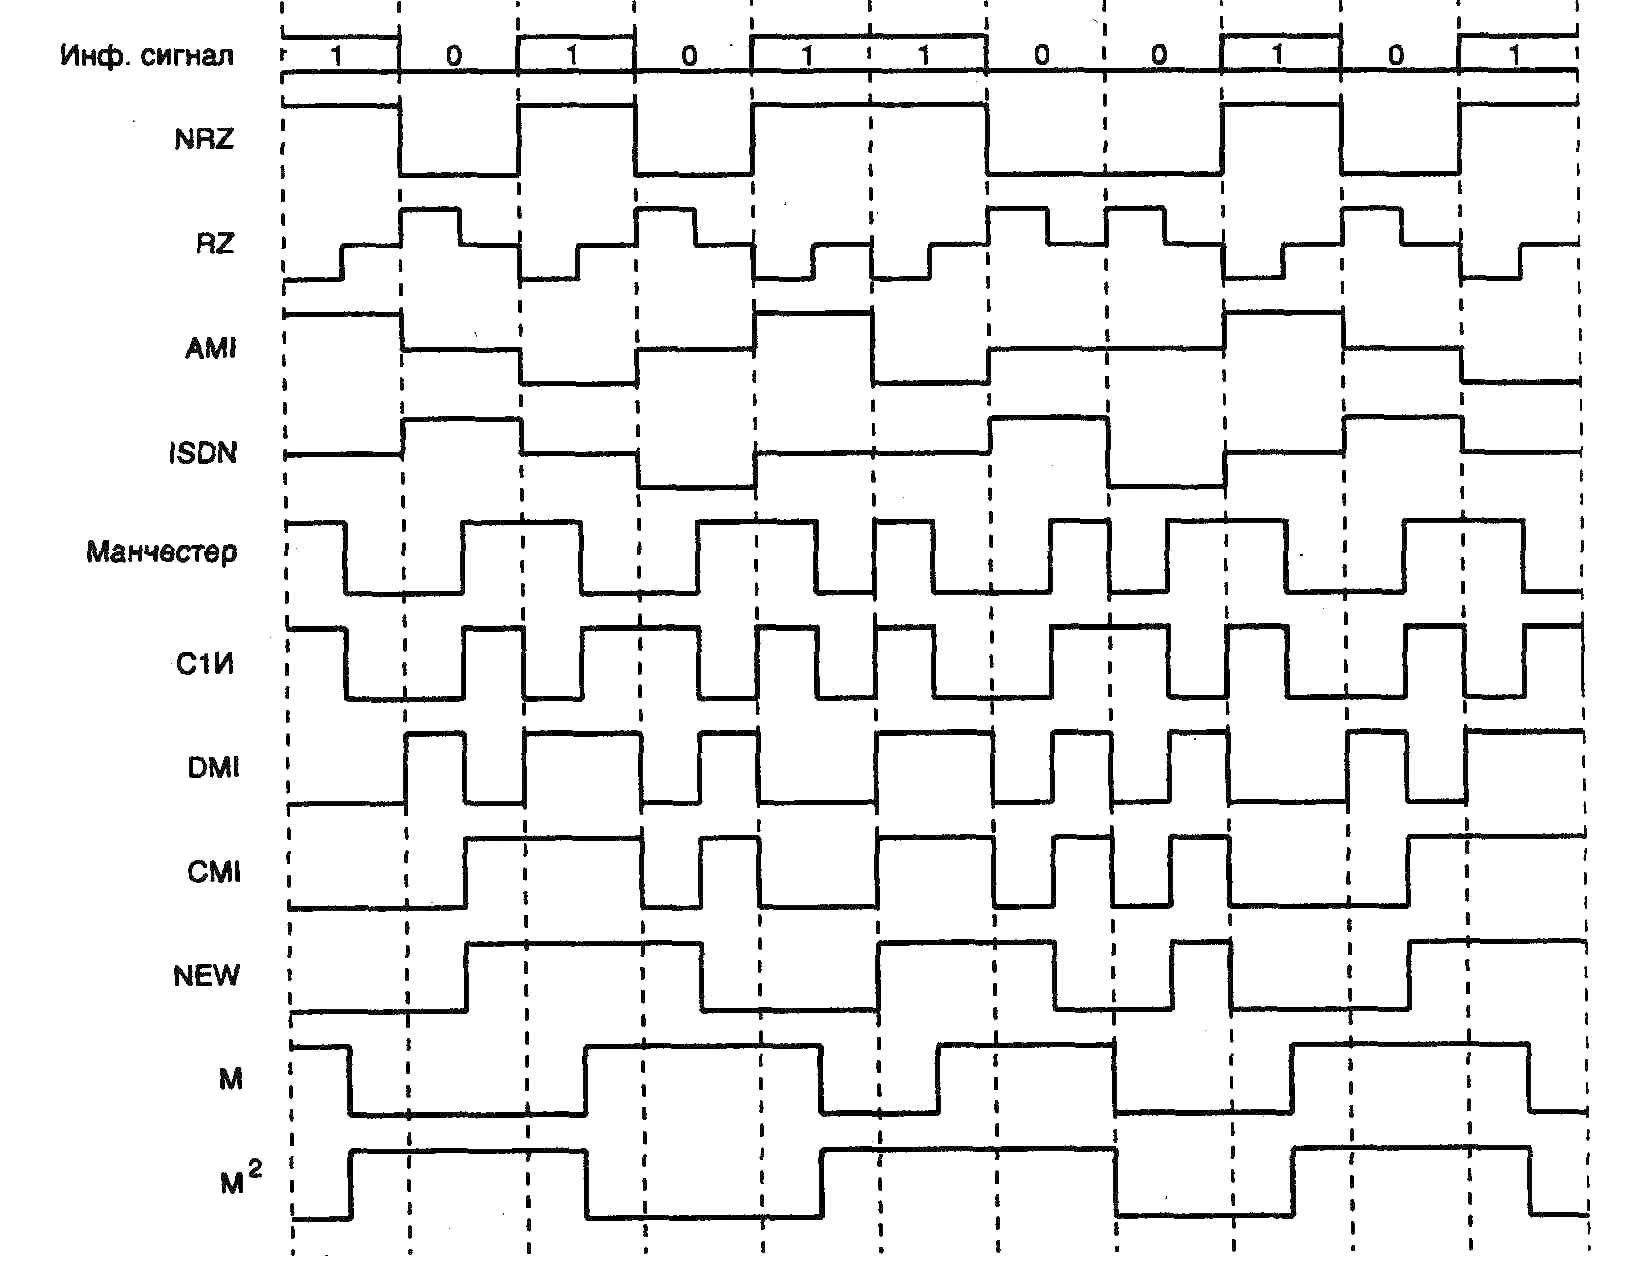
\includegraphics[width=10cm]{11_1}
\begin{center}
Различные системы кодирования данных
\end{center}
\end{minipage}
\\
\subsubsection{Модуляция}
Если сетевая карта умеет генерировать физический сигнал в виде синусоиды, то управляя амплитудой/частотой/фазой этой синусоиды, можно кодировать 0 и 1.
\\
\begin{minipage}{\textwidth}
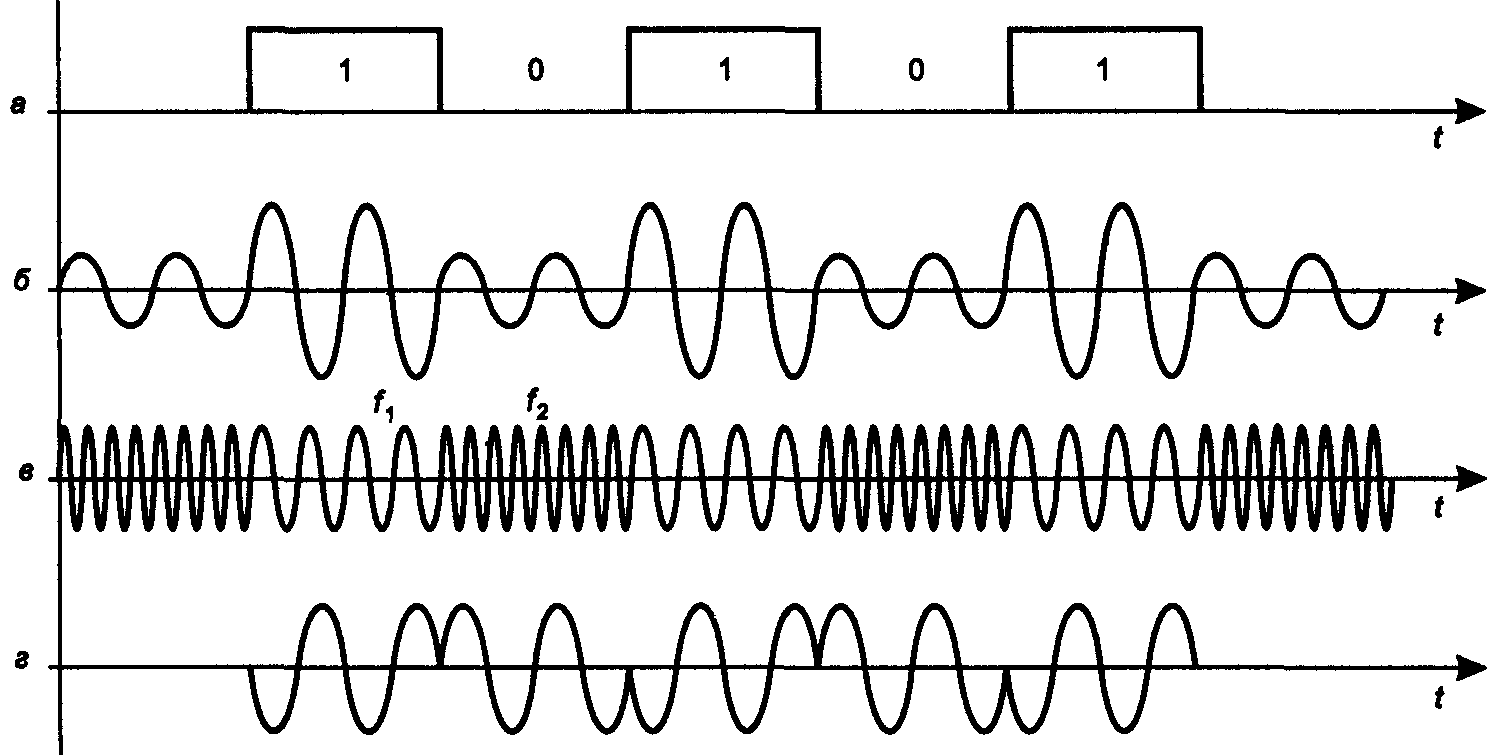
\includegraphics[width=10cm]{11_2}
\begin{center}
а) информационный сигнал, б) амплитудная модуляция (AM), в) частотная модуляция (FM), г) фазовая модуляция (PM)
\end{center}
\end{minipage}
\subsection{Адекватность OSI-модели}
Не существует ни одной сетевой технологии, в которой бы была идеально реализована вся OSI-модель с четким разделением уровней.
Модель OSI далека от реальности, ее назначение - быть идеальной абстракцией.
\begin{table}[!h]
\begin{tabular}{r|l}
Реальность & OSI-уровни \\
\hline
Skype & 7,6,5 \\
\hline
FTP & 7,3 \\
\hline
TCP & 7,5,4,3 \\
\hline
IP & 3,4 \\
\hline
Wi-Fi & 1,2 \\
\hline
Fast-Ethernet & 1,2 \\
\end{tabular}
\end{table}
\section{Отличие TCP от UDP}
\begin{table}[h]
\begin{tabular}{|l|c|c|}
\hline
Свойство & TCP & UDP \\
\hline
Установка соединения & $\checkmark$ & $\times$ \\
Разрыв соединения &  $\checkmark$ & $\times$ \\
Подтверждение доставки &  $\checkmark$ & $\times$ \\
Проверка контрольной суммы  & $\checkmark$ & $\checkmark$ \\
Обнаружение искаженных пакетов & $\checkmark$ & $\checkmark$ \\
Обнаружение потерянных пакетов & $\checkmark$ & $\times$ \\
Повторная передача потерянных/искаженных & $\checkmark$ & $\times$ \\
\hline
\end{tabular}
\end{table}
\textbf{TCP} применяют, если необходимо удостовериться, что все данные дошли корректно, получив об этом подтверждение и организовав повторную передачу поврежденных данных (пример: передача почты).
\\\textbf{UDP} применяют либо если канал связи абсолютно надежен, либо если нет смысла повторно передавать потерянные/искаженные пакеты (пример: видео-звонок), но при этом хочется сэкономить на передаче ненужных служебных данных, используемых в ТСР.
\section{Сетевые устройства}

\begin{minipage}{\textwidth}
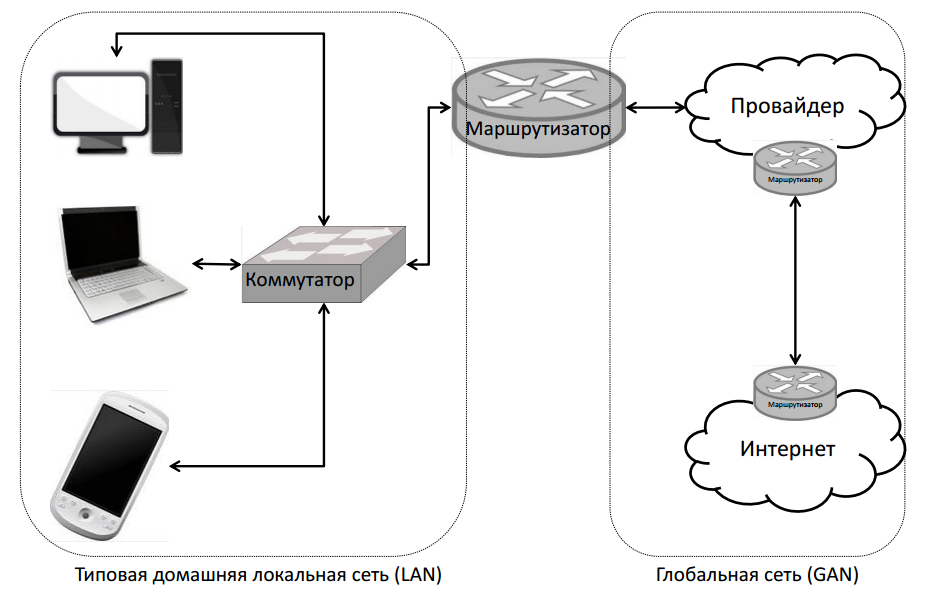
\includegraphics[width=10cm]{11_3}
\end{minipage}

\begin{center}
  \textbf{Сравнение коммутатора и маршрутизатора}
\end{center}

\begin{table}[!h]
 \begin{tabular}{|c|c|c|}
 \hline
 \multirow{2}{*}{Свойство} & Коммутатор & Маршрутизатор \\
 & (switch) & (router) \\
 \hline
 & & Много (ровно по \\
 Наличие MAC-адреса & Нет & по одному на каждый \\
 & & порт/антенну) \\
 \hline
 & & Много (минимум по \\
 Наличие IP-адреса & Нет & по одному на каждый \\
 & &  порт/антенну) \\
 \hline
 Уровни OSI-модели & 1,2 & 1,2,3 \\
 \hline
 Умение выбирать & Нет (так как в локаль-  & \\
 маршруты & ной сети всегда только  & Да\\
 & один маршрут & \\
 \hline
 & Обмен данными между & Обмен данными  \\
 Назначение & компьютерами внутри & между несколькими  \\
 & локальной сети & локальными сетями \\
 \hline
  \end{tabular}
\end{table}
\textbf{Примечание:} существуют гибридные устройства, совмещающие в себе коммутатор и маршрутизатор (они используются у большинства пользователей домашнего интернета, однако в корпоративных сетях применяются реже).
